\documentclass{beamer}
\usepackage{graphicx}
\usepackage{listings}
\usepackage{tikz}
\usetikzlibrary{positioning, arrows.meta, shapes, calc, shapes.multipart}

\title{Introducing Qubes Air design}
\author{Marek Marczykowski-Górecki and Frédéric Pierret}
\date{September 20, 2024}

\begin{document}

\frame{\titlepage}


\begin{frame}{Overview}
    \begin{itemize}
        \item Understanding communication between Qubes OS hosts.
        \item Different classes involved in the communication process.
        \item RPC requests and policy processing.
        \item Relay mechanisms for remote communication.
    \end{itemize}
\end{frame}

\begin{frame}{Classes}
    \begin{itemize}
        \item The communication uses the following classes:
        \begin{itemize}
            \item \textbf{BaseVM}: The base class for all VMs.
            \item \textbf{LocalVM}: Represents a VM on the local QubesOS.
            \item \textbf{RemoteVM}: Represents a VM on a remote QubesOS.
            \item \textbf{RelayVM(RemoteVM)}: Acts as a relay for communication with remote VMs.
        \end{itemize}
    \end{itemize}
\end{frame}

\begin{frame}{General Case}
    \begin{itemize}
        \item Communication sequence between local and remote QubesOS:
    \end{itemize}
    \begin{center}
        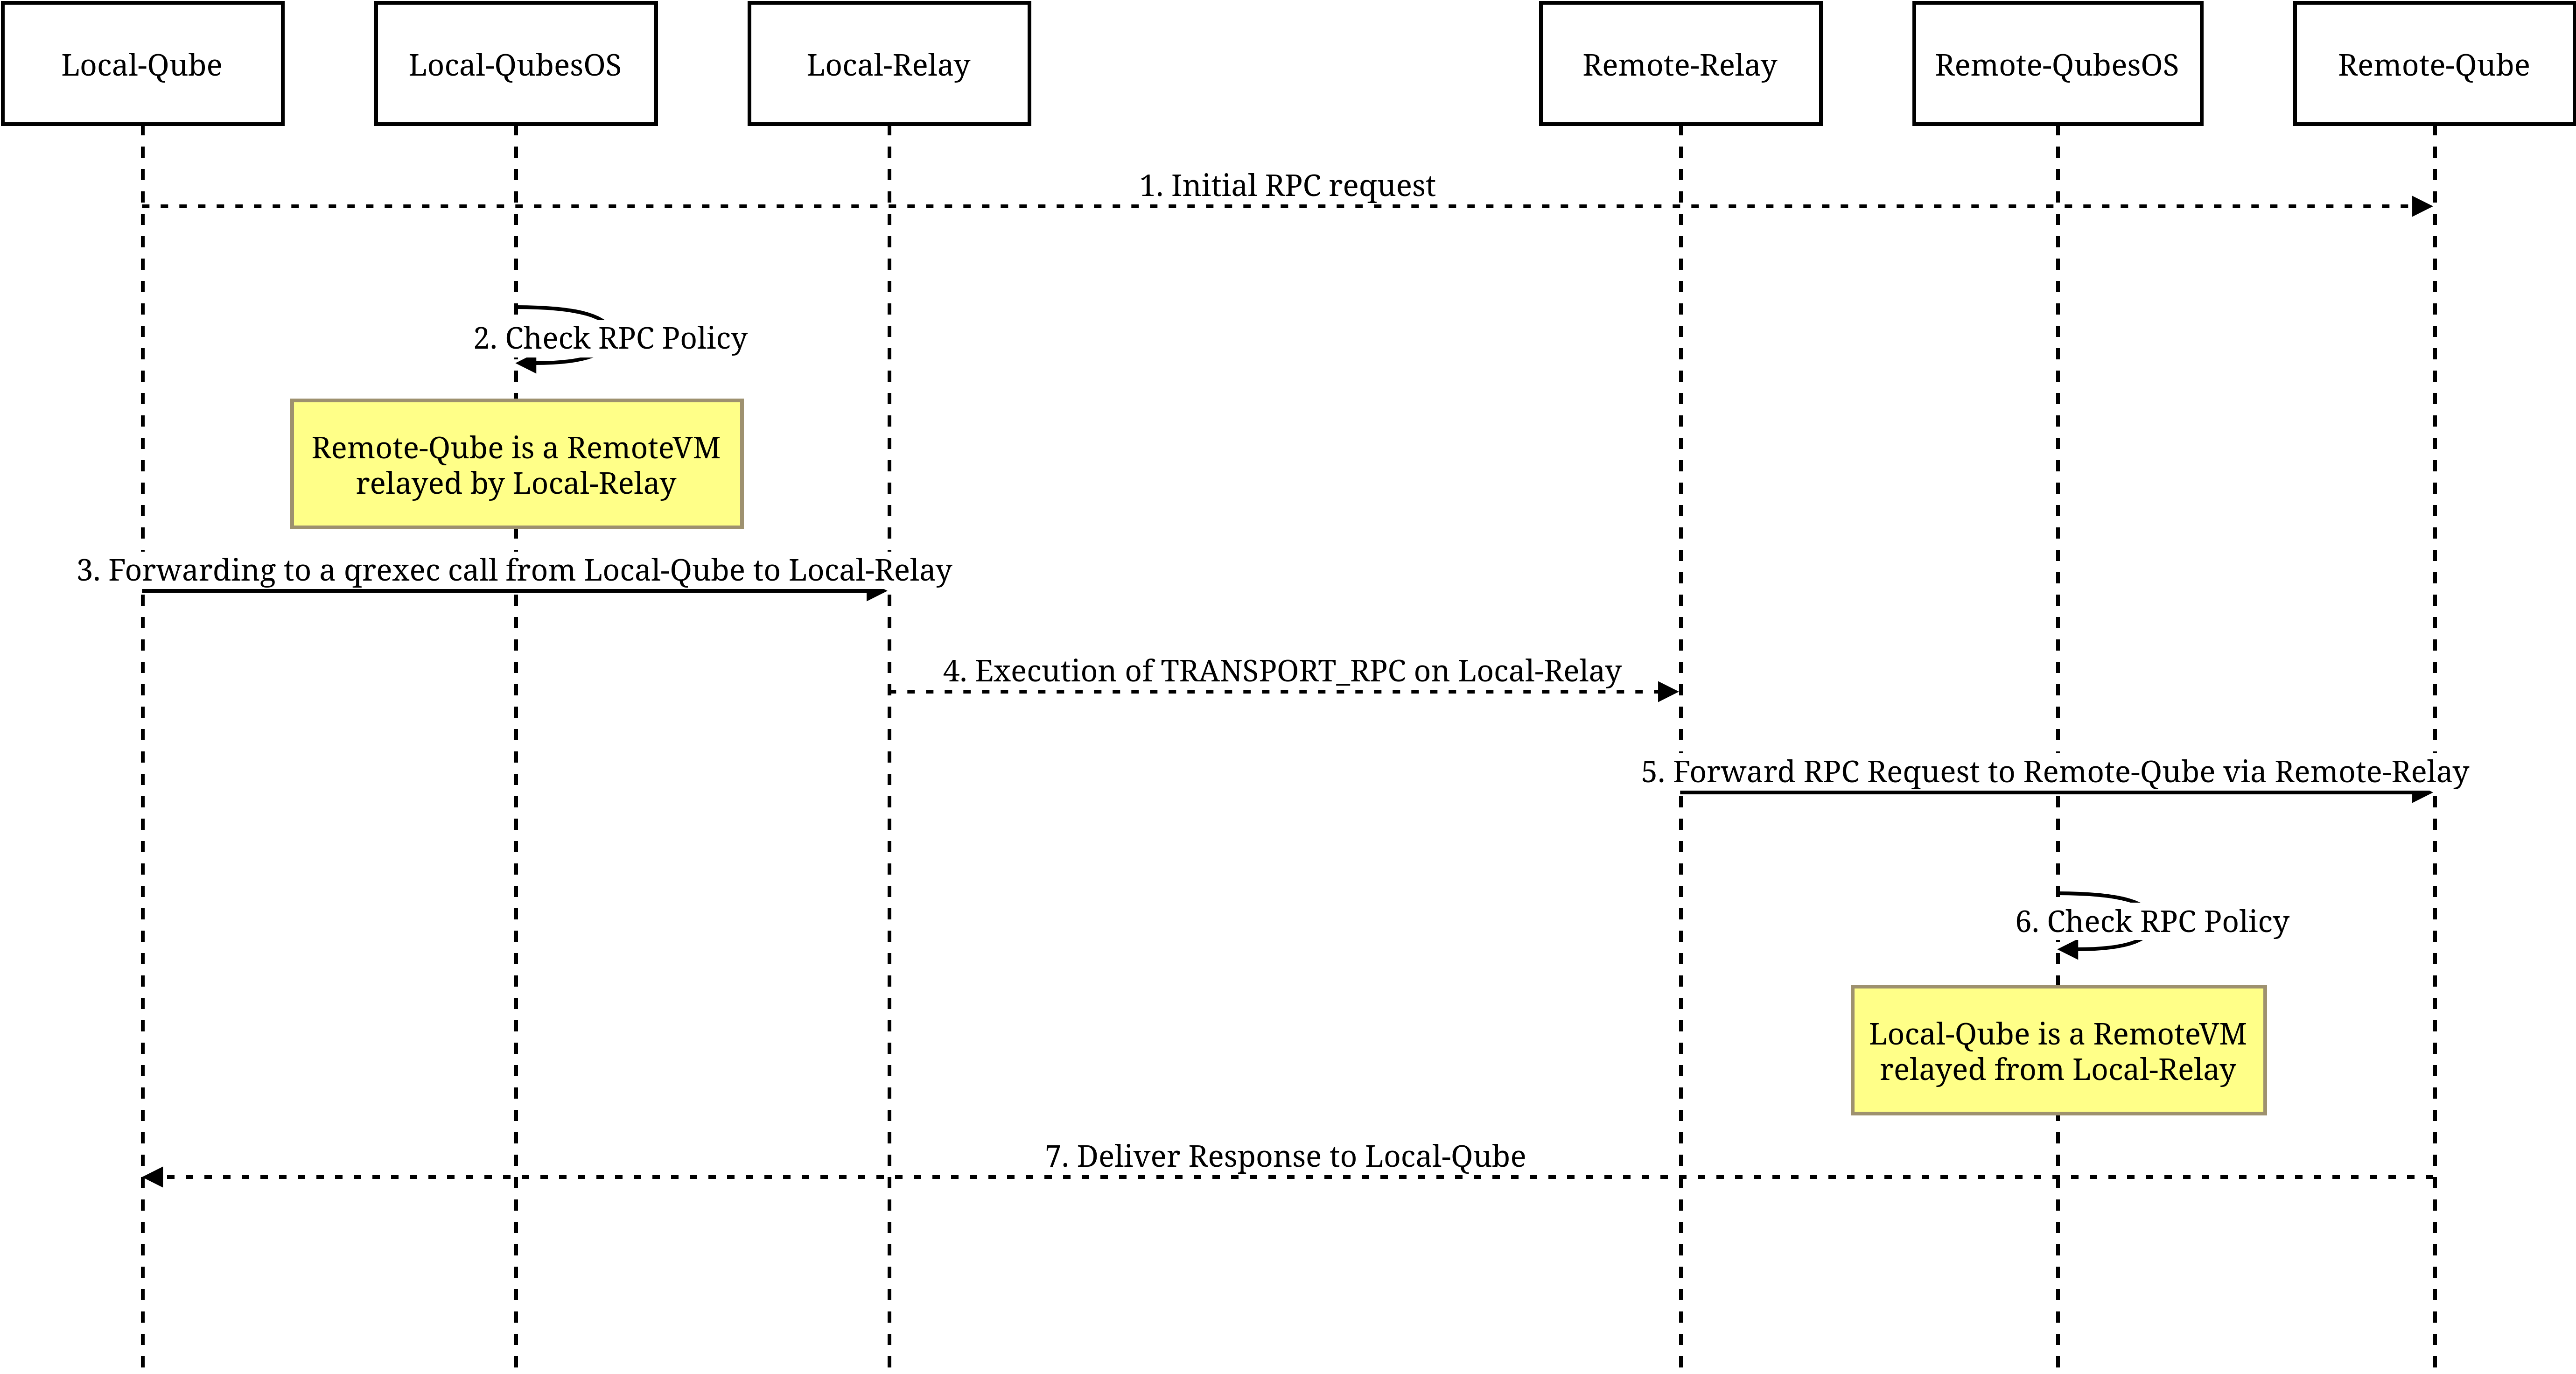
\includegraphics[width=\linewidth]{general.png}
    \end{center}
\end{frame}


\begin{frame}{Particular Case: Non-QubesOS Host RemoteVM}
    \begin{itemize}
        \item RemoteVM can be on standard Linux or Windows machines, RPi, etc.
        \item Useful for interaction with other virtual machines (e.g. KVM VMs).
    \end{itemize}
	\begin{center}
        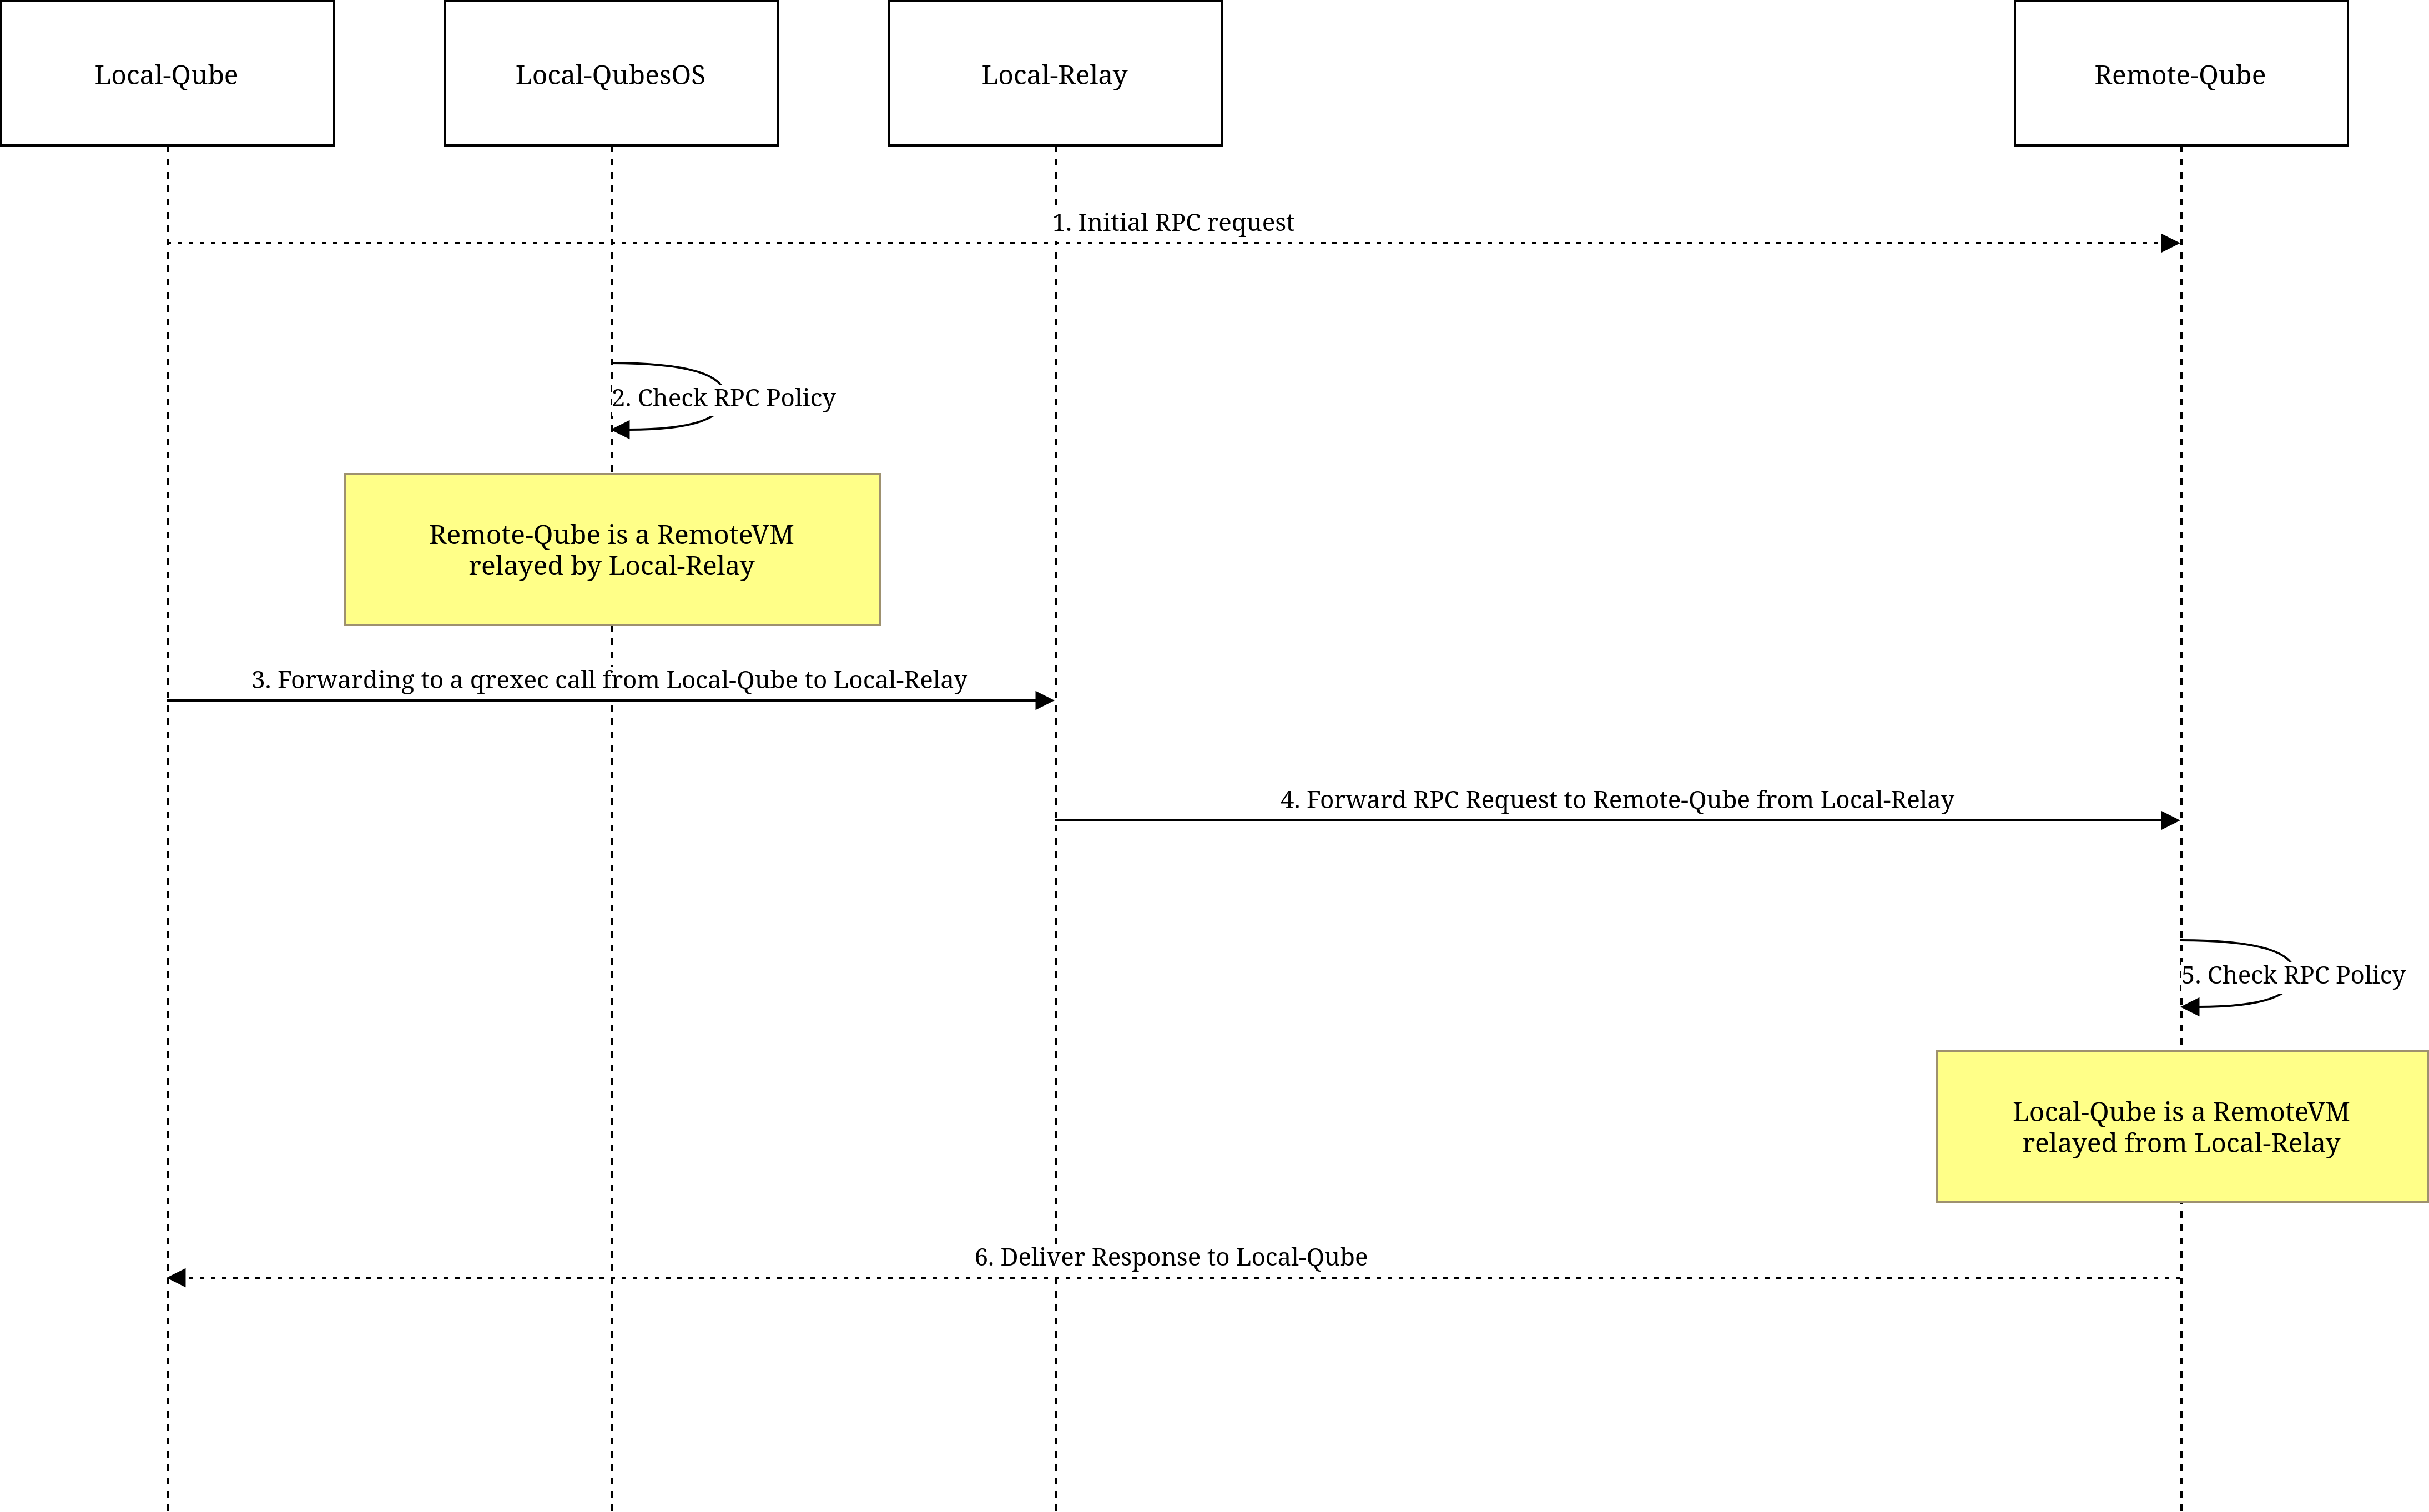
\includegraphics[width=\linewidth]{particular.png}
    \end{center}
\end{frame}

\begin{frame}{Summary}
    \begin{itemize}
        \item The process involves multiple relays and policy checks to ensure secure communication.
        \item Potential improvements include end-to-end verification and handling of unknown connections.
    \end{itemize}
\end{frame}

\end{document}
